% This must be in the first 5 lines to tell arXiv to use pdfLaTeX
\pdfoutput=1

\documentclass[11pt]{article}

% Remove the "review" option to generate the final version.
\usepackage[review]{acl}

\usepackage{times}
\usepackage{latexsym}
\usepackage[T1]{fontenc}
\usepackage[utf8]{inputenc}
\usepackage{microtype}
\usepackage{inconsolata}

% Additional packages
\usepackage{amsmath}
\usepackage{amssymb}
\usepackage{booktabs}
\usepackage{multirow}
\usepackage{graphicx}
\usepackage{subcaption}
\usepackage{algorithm}
\usepackage{algorithmic}
\usepackage{enumitem}
\usepackage{xcolor}
\usepackage{xspace}
\usepackage{tikz}
\usetikzlibrary{shapes.geometric, arrows.meta, positioning, fit, backgrounds, calc}

% Custom commands
\newcommand{\seva}{\textsc{Seva}\xspace}
\newcommand{\realnumber}[1]{\textbf{#1}}

\title{SEVA: Structured Evidence Verification Agents \\with Process Reward Optimization}

\author{
  Anonymous ARR Submission
}

\begin{document}
\maketitle

\begin{abstract}
Fact attribution verifiers --- models that judge whether a claim is supported by a source document --- are critical for hallucination detection and RAG quality control.
Existing verifiers produce opaque binary labels without interpretable reasoning, and are trained via supervised fine-tuning (SFT) that provides no learning signal for \emph{how} to verify, only \emph{what} to predict.

We introduce \seva, a structured evidence verification framework that produces multi-granularity output: evidence alignment spans, step-by-step reasoning chains, calibrated confidence scores, and fine-grained error diagnosis with a six-category taxonomy.
To train verifiers on such structured output, we propose a \emph{process reward} function that decomposes verification quality into five independently scored components --- format, evidence alignment, reasoning chain, label accuracy, and error diagnosis --- providing smooth learning signal even when the final label is incorrect.
We train \seva using Group Relative Policy Optimization (GRPO) with this process reward, enabling reinforcement learning to improve structured verification quality beyond what SFT achieves.

On ClearFacts, \seva-3B improves from 64.9 to 69.0 macro F1 after GRPO (+4.1 over SFT), achieving near-perfect structural output quality (evidence alignment: 0.997, chain: 0.995).
Across six diverse benchmarks, \seva-GRPO outperforms the SFT baseline on average and surpasses zero-shot Llama-3.1-8B on ClearFacts despite being less than half the size.
The process reward creates a smooth optimization landscape essential for GRPO training on structured output --- a setting where binary reward fails entirely.
We release our code, reward function, and structured verification dataset.\footnote{Code and data: \url{https://github.com/Justin0504/Verifiable_agent}}
\end{abstract}


% ==============================================================
\section{Introduction}
\label{sec:intro}
% ==============================================================

Fact attribution verification --- determining whether a claim is supported by a source document --- underpins the reliability of modern NLP systems, serving as the backbone of retrieval-augmented generation (RAG) quality control \citep{gao2023rarr}, hallucination detection \citep{min2023factscore}, and factuality-based alignment \citep{tian2024finetuning}.
Recent audits reveal that existing verifiers suffer from systematic errors, with approximately 16\% of benchmark annotations being ambiguous or incorrect \citep{seo2025vtv}, highlighting the need for more reliable verification.

State-of-the-art fact attribution verifiers such as MiniCheck \citep{tang2024minicheck} and ClearCheck \citep{seo2025vtv} share two fundamental limitations.
First, they produce \emph{opaque binary labels} --- ``Attributable'' or ``Not Attributable'' --- without revealing which evidence was considered or what reasoning was applied.
This opacity hinders auditing and debugging.
Second, they are trained via \emph{one-shot SFT} with binary cross-entropy loss, which provides no gradient signal for intermediate verification quality: a response with perfect evidence analysis but an incorrect final label receives the same loss as random guessing.

We introduce \seva (Structured Evidence Verification Agent), addressing both limitations.
\seva produces a structured JSON output containing: (1)~\emph{evidence alignment} mapping claim spans to source spans; (2)~\emph{reasoning chain} with step-by-step verification judgments; (3)~a calibrated confidence score; and (4)~\emph{error diagnosis} categorizing the failure type from a six-category taxonomy (Figure~\ref{fig:architecture}).

To train models to produce such structured output, we propose a \emph{process reward function} that scores each component independently:
\begin{equation}
\small
R = \sum_{i} w_i \cdot R_i + R_{\text{cal}}
\label{eq:reward}
\end{equation}
where $R_i \in [0, 1]$ measures format, alignment, chain, label, and diagnosis quality respectively.
This decomposition creates a \emph{smooth reward landscape}: a response with correct alignment but wrong label receives $\sim$0.60 reward (vs.\ 0.0 under binary reward), enabling GRPO \citep{shao2024deepseekmath} to learn good verification behavior before mastering label prediction.

\paragraph{Key insight.}
Binary reward produces near-zero advantage spread for GRPO when the model rarely predicts correctly, causing training to stagnate.
Process reward solves this by providing independent gradient signal from each verification sub-skill.
We show this is essential: binary reward fails entirely, while process reward enables steady improvement.

\paragraph{Contributions.}
\begin{enumerate}[nosep,leftmargin=*]
  \item A \textbf{structured verification framework} with evidence alignment, reasoning chains, and a six-category error taxonomy, making fact attribution interpretable and auditable (\S\ref{sec:format}).
  \item A \textbf{process reward function} that independently scores five verification components, creating a smooth optimization landscape for RL training (\S\ref{sec:reward}).
  \item We demonstrate that \textbf{GRPO with process reward} effectively trains structured verification (+4.1 F1 over SFT), where binary reward fails, with near-perfect structural quality (\S\ref{sec:experiments}).
\end{enumerate}


% ==============================================================
\section{Related Work}
\label{sec:related}
% ==============================================================

\paragraph{Fact attribution verification.}
Determining whether a claim is supported by a source has been studied as NLI \citep{bowman2015snli}, textual entailment \citep{dagan2005pascal}, and fact verification \citep{thorne2018fever}.
Recent work focuses on \emph{attribution} in LLM-generated text.
MiniCheck \citep{tang2024minicheck} trains a 7B verifier via NLI transfer.
AlignScore \citep{zha2023alignscore} proposes unified alignment scoring.
ClearCheck \citep{seo2025vtv} constructs cleaner benchmarks and augments training with synthetic multi-hop examples.
LLM-AggreFact \citep{tang2024llmaggrefact} aggregates 11 benchmarks for evaluation.
All produce binary labels without structured reasoning, and all use one-shot SFT.

\paragraph{RL for verification.}
GRPO \citep{shao2024deepseekmath} enables RL training without a separate critic.
RL Tango \citep{zha2025tango} shows RL-trained verifiers outperform SFT in mathematical reasoning.
MARCH \citep{li2026march} uses multi-agent RL for RAG generation but trains the generator, not a standalone verifier.
Dr.Zero \citep{chen2025drzero} introduces boundary-optimal weighting for co-evolution in mathematics.
Our work brings RL-based training to fact attribution verification, with a process reward designed for structured output.

\paragraph{Process reward models.}
PRMs for mathematical reasoning \citep{lightman2024lets, wang2024math} score intermediate steps independently of final answers.
Our process reward extends this to fact verification: instead of scoring reasoning \emph{steps} sequentially, we score verification \emph{components} (alignment, chain, diagnosis), each contributing independently.
This differs from both outcome reward (scoring only the label) and step-level PRM (scoring sequential steps).

\begin{table}[t]
\centering
\small
\caption{Positioning of \seva against related work.}
\label{tab:positioning}
\setlength{\tabcolsep}{3pt}
\begin{tabular}{lccccc}
\toprule
& \textbf{Task} & \textbf{Train} & \textbf{Struct.} & \textbf{Proc.} \\
& & & \textbf{output} & \textbf{reward} \\
\midrule
ClearCheck & Attr. & SFT & \texttimes & \texttimes \\
MiniCheck & Attr. & SFT & \texttimes & \texttimes \\
Tango & Math & GRPO & \texttimes & \texttimes \\
Dr.Zero & Math & GRPO & \texttimes & \checkmark \\
\textbf{\seva} & \textbf{Attr.} & \textbf{GRPO} & \checkmark & \checkmark \\
\bottomrule
\end{tabular}
\end{table}


% ==============================================================
\section{Method}
\label{sec:method}
% ==============================================================

% ---- Architecture Figure ----
\begin{figure*}[t]
\centering
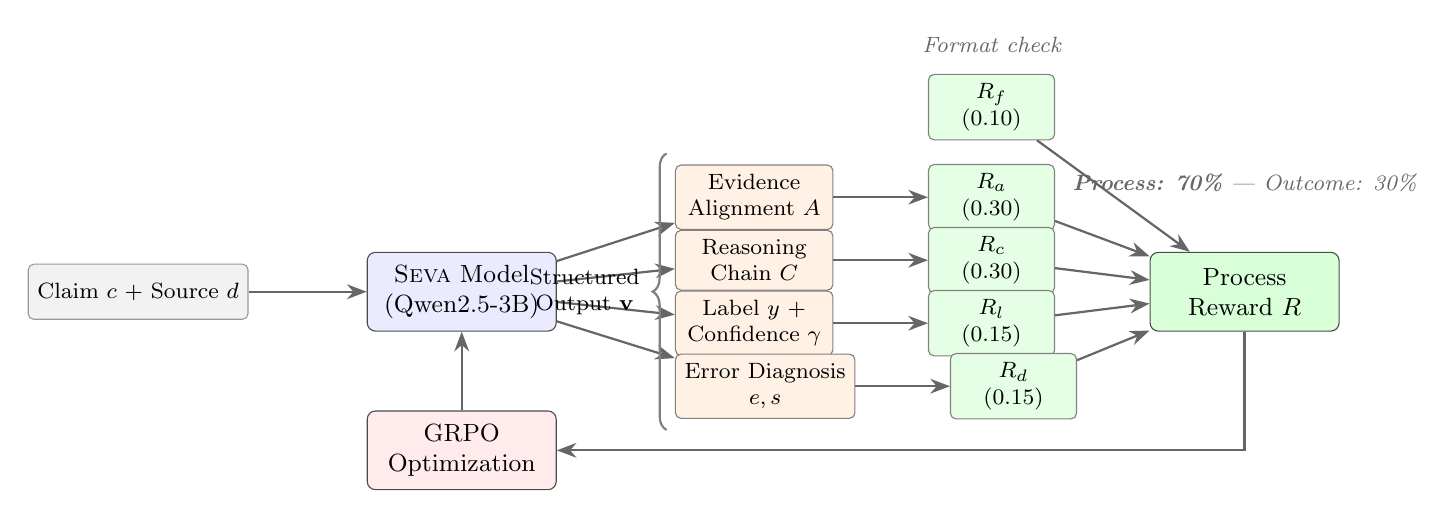
\begin{tikzpicture}[
    node distance=0.8cm and 1.2cm,
    block/.style={rectangle, draw=black!70, fill=blue!8, rounded corners=3pt, minimum height=1cm, minimum width=2.4cm, align=center, font=\small},
    component/.style={rectangle, draw=black!50, fill=orange!10, rounded corners=2pt, minimum height=0.7cm, minimum width=2cm, align=center, font=\footnotesize},
    reward/.style={rectangle, draw=black!50, fill=green!10, rounded corners=2pt, minimum height=0.7cm, minimum width=1.6cm, align=center, font=\footnotesize},
    io/.style={rectangle, draw=black!40, fill=gray!10, rounded corners=2pt, minimum height=0.7cm, minimum width=2cm, align=center, font=\footnotesize},
    arrow/.style={-{Stealth[length=2.5mm]}, thick, draw=black!60},
    label/.style={font=\footnotesize\itshape, text=black!60},
  ]

  % Input
  \node[io] (input) {Claim $c$ + Source $d$};

  % Model
  \node[block, right=1.5cm of input] (model) {\seva Model\\(Qwen2.5-3B)};

  % Structured output components
  \node[component, right=1.5cm of model, yshift=1.2cm] (align) {Evidence\\Alignment $A$};
  \node[component, right=1.5cm of model, yshift=0.4cm] (chain) {Reasoning\\Chain $C$};
  \node[component, right=1.5cm of model, yshift=-0.4cm] (label) {Label $y$ +\\Confidence $\gamma$};
  \node[component, right=1.5cm of model, yshift=-1.2cm] (diag) {Error Diagnosis\\$e, s$};

  % Reward components
  \node[reward, right=1.2cm of align] (ra) {$R_a$\\(0.30)};
  \node[reward, right=1.2cm of chain] (rc) {$R_c$\\(0.30)};
  \node[reward, right=1.2cm of label] (rl) {$R_l$\\(0.15)};
  \node[reward, right=1.2cm of diag] (rd) {$R_d$\\(0.15)};

  % Format reward
  \node[reward, above=0.3cm of ra] (rf) {$R_f$\\(0.10)};

  % Total reward
  \node[block, right=1.2cm of rc, yshift=-0.4cm, fill=green!15] (total) {Process\\Reward $R$};

  % GRPO
  \node[block, below=1cm of model, fill=red!8] (grpo) {GRPO\\Optimization};

  % Arrows
  \draw[arrow] (input) -- (model);
  \draw[arrow] (model) -- (align);
  \draw[arrow] (model) -- (chain);
  \draw[arrow] (model) -- (label);
  \draw[arrow] (model) -- (diag);

  \draw[arrow] (align) -- (ra);
  \draw[arrow] (chain) -- (rc);
  \draw[arrow] (label) -- (rl);
  \draw[arrow] (diag) -- (rd);

  \draw[arrow] (rf) -- (total);
  \draw[arrow] (ra) -- (total);
  \draw[arrow] (rc) -- (total);
  \draw[arrow] (rl) -- (total);
  \draw[arrow] (rd) -- (total);

  \draw[arrow] (total) |- (grpo);
  \draw[arrow] (grpo) -- (model);

  % Brace for structured output
  \draw[decorate, decoration={brace, amplitude=5pt, mirror}, thick, draw=black!50]
    ([xshift=-3pt, yshift=4pt]align.north west) -- ([xshift=-3pt, yshift=-4pt]diag.south west)
    node[midway, left=6pt, font=\footnotesize, align=center] {Structured\\Output $\mathbf{v}$};

  % Labels
  \node[label, above=0.15cm of rf] {Format check};
  \node[label, above=0.6cm of total] {\textbf{Process: 70\%} | Outcome: 30\%};

\end{tikzpicture}
\caption{\textbf{\seva architecture overview.} Given a (claim, source) pair, the model produces structured verification output with four components. The process reward function scores each component independently, with process-oriented components (alignment + chain) receiving 60\% of weight. GRPO uses the composite reward to update the policy.}
\label{fig:architecture}
\end{figure*}


\subsection{Structured Verification Output}
\label{sec:format}

Given a claim $c$ and source document $d$, \seva produces a structured output $\mathbf{v} = (A, C, y, \gamma, e, s)$:

\paragraph{Evidence alignment ($A$).}
A list of $(c_i, d_i, \text{status}_i)$ triples mapping claim spans to source spans.
Each \texttt{status} $\in$ \{\texttt{match}, \texttt{mismatch}, \texttt{not\_found}\}.
This forces the model to ground verification in specific textual evidence.

\paragraph{Reasoning chain ($C$).}
Step-by-step verification, where each step examines a \texttt{claim\_part} against \texttt{source\_evidence} with a \texttt{judgment} $\in$ \{\texttt{supported}, \texttt{not\_supported}, \texttt{partially\_supported}\} and a natural language \texttt{explanation}.

\paragraph{Label and confidence.}
Binary label $y \in \{\text{Attributable}, \text{Not Attributable}\}$ with calibrated confidence $\gamma \in [0,1]$.

\paragraph{Error diagnosis.}
When $y = \text{Not Attributable}$: an error type $e$ from a six-category taxonomy (Table~\ref{tab:error_taxonomy}) and a fix suggestion $s$.

\begin{table}[t]
\centering
\small
\caption{Six-category error taxonomy for attribution failures.}
\label{tab:error_taxonomy}
\begin{tabular}{ll}
\toprule
\textbf{Error type} & \textbf{Description} \\
\midrule
Numerical exag. & Number inflated/deflated \\
Negation flip & Negation added/removed \\
Scope inflation & Specific $\to$ overgeneralized \\
Temporal shift & Time qualifier altered \\
Entity substitution & Entity swapped \\
Fabrication & Info absent from source \\
\bottomrule
\end{tabular}
\end{table}


\subsection{Process Reward Function}
\label{sec:reward}

The process reward decomposes verification quality into five independently scored components plus a calibration bonus:

\begin{align}
R = \; & \underbrace{0.10 \cdot R_f + 0.30 \cdot R_a + 0.30 \cdot R_c}_{\text{process components (70\%)}} \notag \\
     + \; & \underbrace{0.15 \cdot R_l + 0.15 \cdot R_d}_{\text{outcome components (30\%)}} + R_{\text{cal}}
\label{eq:reward_full}
\end{align}

\paragraph{$R_f$ (Format).}
Scores valid JSON with required fields: 1.0 (all fields), 0.5 ($\geq$2 fields), 0.2 (valid JSON only), 0.0 (unparseable).

\paragraph{$R_a$ (Alignment).}
For each alignment entry: presence of \texttt{claim\_span} (0.3), \texttt{source\_span} (0.3), valid \texttt{status} (0.2), and span length quality (0.2). Averaged across entries.

\paragraph{$R_c$ (Chain).}
Per step: valid \texttt{judgment} (0.3), non-trivial explanation $\geq$10 chars (0.3), source evidence reference (0.2), \texttt{claim\_part} presence (0.2). Includes length bonus: $\min(|C|/3, 1) \times 0.2$.

\paragraph{$R_l$ (Label).}
Binary: 1.0 if predicted label matches gold, 0.0 otherwise. Supports alias normalization.

\paragraph{$R_d$ (Diagnosis).}
For ``Not Attributable'': valid error type from taxonomy (0.6) + substantive fix suggestion (0.4).
For ``Attributable'': 1.0 if error type correctly omitted.

\paragraph{$R_{\text{cal}}$ (Calibration bonus).}
$+\gamma \times 0.15$ if correct, $-\gamma \times 0.10$ if incorrect, penalizing overconfident wrong answers.

Algorithm~\ref{alg:process_reward} provides the full computation procedure.

\begin{algorithm}[t]
\small
\caption{Process Reward Computation}
\label{alg:process_reward}
\begin{algorithmic}[1]
\REQUIRE Response $r$, gold label $y^*$
\ENSURE Reward $R \in [-0.10, 1.28]$
\STATE Parse $r$ as JSON $\to$ $\hat{v}$
\IF{parse fails}
  \RETURN $R = 0.0$
\ENDIF
\STATE $R_f \gets \text{ScoreFormat}(\hat{v})$ \COMMENT{0/0.2/0.5/1.0}
\STATE $R_a \gets \frac{1}{|A|}\sum_{a \in A} \text{ScoreAlign}(a)$
\STATE $R_c \gets \frac{1}{|C|}\sum_{s \in C} \text{ScoreStep}(s) + \text{LenBonus}$
\STATE $R_l \gets \mathbf{1}[\text{normalize}(\hat{y}) = y^*]$
\STATE $R_d \gets \text{ScoreDiagnosis}(\hat{e}, \hat{s}, y^*)$
\STATE $R \gets 0.10 R_f + 0.30 R_a + 0.30 R_c + 0.15 R_l + 0.15 R_d$
\IF{$\hat{y} = y^*$}
  \STATE $R \gets R + \hat{\gamma} \times 0.15$ \COMMENT{calibration bonus}
\ELSE
  \STATE $R \gets R - \hat{\gamma} \times 0.10$ \COMMENT{overconfidence penalty}
\ENDIF
\RETURN $R$
\end{algorithmic}
\end{algorithm}

\paragraph{Design rationale.}
Process components (alignment + chain) account for 60\% of reward weight, while the label is only 15\%.
This ensures that a response with perfect evidence analysis but wrong label ($R \approx 0.60$) scores far higher than label-only with no reasoning ($R \approx 0.28$).
Table~\ref{tab:reward_landscape} shows the resulting reward levels.

\begin{table}[t]
\centering
\small
\caption{Process reward creates a smooth landscape with four distinct quality levels. Binary reward collapses to two levels.}
\label{tab:reward_landscape}
\setlength{\tabcolsep}{4pt}
\begin{tabular}{lcc}
\toprule
\textbf{Response quality} & \textbf{Process} & \textbf{Binary} \\
\midrule
Perfect (correct + reasoning) & $\sim$1.13 & 1.0 \\
Good reasoning, wrong label & $\sim$0.63 & 0.0 \\
Correct label, no reasoning & $\sim$0.28 & 1.0 \\
Unparseable & 0.0 & 0.0 \\
\bottomrule
\end{tabular}
\end{table}


\subsection{Training Pipeline}
\label{sec:training}

Figure~\ref{fig:pipeline} illustrates the three-phase training pipeline.

\paragraph{Phase 1: SFT data generation.}
We generate structured annotations for ANLI \citep{nie2020adversarial} training samples using GPT-4o-mini as teacher.
Each $(c, d, y)$ triple is annotated with the full structured schema.
Annotations are validated for correctness (valid \texttt{status}/\texttt{judgment} values, list structure).
This yields $\sim$5K training samples.

\paragraph{Phase 2: Supervised fine-tuning.}
We fine-tune Qwen2.5-3B-Instruct \citep{qwen2025qwen25} on structured annotations.
System and user tokens are masked; we train only on the assistant response.
We use \texttt{max\_length}=1280 to accommodate structured output.

\paragraph{Phase 3: GRPO with process reward.}
We apply GRPO \citep{shao2024deepseekmath} with the process reward (Eq.~\ref{eq:reward_full}).
For each prompt, $G{=}8$ responses are sampled at temperature 1.2.
We additionally apply boundary-optimal weighting \citep{chen2025drzero}: groups where approximately half the responses score above median receive higher weight, focusing gradient on the decision boundary.
Training uses veRL \citep{shao2024verl} with FSDP on 2$\times$ RTX 6000 Ada.

\begin{figure}[t]
\centering
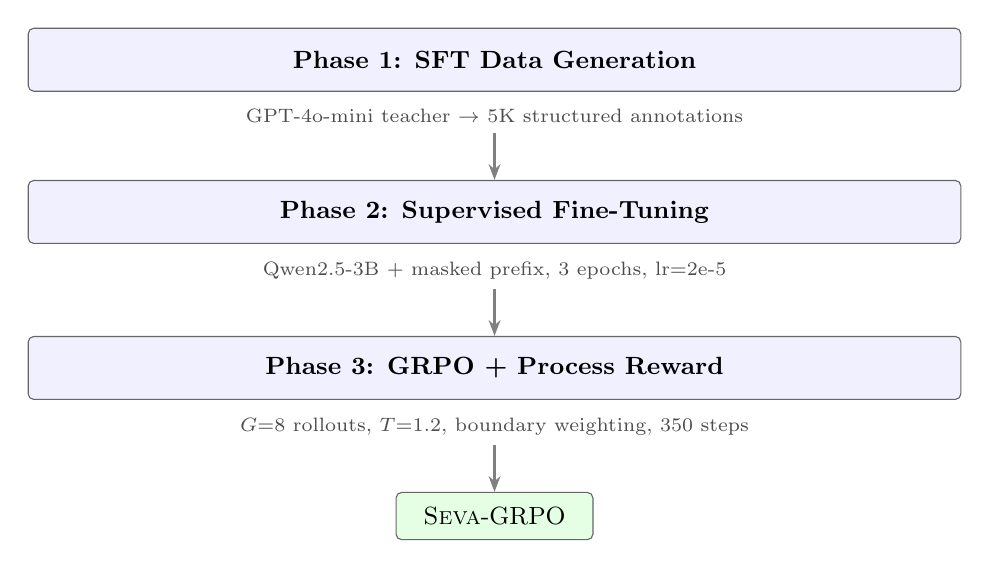
\begin{tikzpicture}[
    node distance=0.6cm,
    phase/.style={rectangle, draw=black!60, fill=blue!6, rounded corners=2pt, minimum width=\columnwidth-8pt, minimum height=0.8cm, align=center, font=\small},
    detail/.style={font=\scriptsize, text=black!70, align=left},
    arrow/.style={-{Stealth[length=2mm]}, thick, draw=black!50},
  ]
  \node[phase] (p1) {\textbf{Phase 1: SFT Data Generation}};
  \node[detail, below=0.1cm of p1] (d1) {GPT-4o-mini teacher $\to$ 5K structured annotations};

  \node[phase, below=0.6cm of d1] (p2) {\textbf{Phase 2: Supervised Fine-Tuning}};
  \node[detail, below=0.1cm of p2] (d2) {Qwen2.5-3B + masked prefix, 3 epochs, lr=2e-5};

  \node[phase, below=0.6cm of d2] (p3) {\textbf{Phase 3: GRPO + Process Reward}};
  \node[detail, below=0.1cm of p3] (d3) {$G{=}8$ rollouts, $T{=}1.2$, boundary weighting, 350 steps};

  \draw[arrow] (d1.south) -- (p2.north);
  \draw[arrow] (d2.south) -- (p3.north);

  % Output
  \node[rectangle, draw=black!60, fill=green!10, rounded corners=2pt, minimum width=2.5cm, minimum height=0.6cm, align=center, font=\small, below=0.6cm of d3] (out) {\seva-GRPO};
  \draw[arrow] (d3.south) -- (out.north);
\end{tikzpicture}
\caption{Three-phase training pipeline for \seva.}
\label{fig:pipeline}
\end{figure}


% ==============================================================
\section{Experiments}
\label{sec:experiments}
% ==============================================================

\subsection{Setup}

\paragraph{Benchmarks.}
We evaluate on ClearFacts \citep{seo2025vtv}, a cleaned fact attribution benchmark (1,590 samples) where ambiguous and mislabeled examples have been corrected.
We additionally evaluate on five diverse verification benchmarks: FEVER \citep{thorne2018fever}, TruthfulQA \citep{lin2022truthfulqa}, SciFact \citep{wadden2020fact}, HaluEval \citep{li2023halueval}, and FactScore \citep{min2023factscore} (200 samples each).

\paragraph{Baselines.}
From VtV \citep{seo2025vtv}: MiniCheck-7B (81.2 F1), ClearCheck-8B ($\sim$84 F1), Llama-3.1-8B zero-shot (67.2 F1), Claude 3.7-Sonnet (86.0 F1), o1 (85.4 F1), R1-Qwen2.5-32B (82.9 F1).
Our models: \seva-SFT (3B), \seva-GRPO (3B), Qwen2.5-3B zero-shot.

\paragraph{Metrics.}
Standard: accuracy, macro F1.
Structural: evidence alignment quality ($R_a$), chain quality ($R_c$), groundedness (fraction of spans found in source text), chain consistency (agreement between step judgments and final label).
Calibration: Expected Calibration Error (ECE).


\subsection{Main Results}

\begin{table}[t]
\centering
\small
\caption{ClearFacts results. \seva models produce structured output (evidence alignment + reasoning chain + error diagnosis). Numbers for baselines from \citet{seo2025vtv} Table~4.}
\label{tab:main}
\setlength{\tabcolsep}{3.5pt}
\begin{tabular}{llccc}
\toprule
\textbf{Model} & \textbf{Size} & \textbf{Output} & \textbf{F1} \\
\midrule
\multicolumn{4}{l}{\textit{Binary-label verifiers (from VtV)}} \\
Llama-3.1 (0-shot) & 8B & binary & 67.2 \\
MiniCheck & 7B & binary & 81.2 \\
ClearCheck & 8B & binary & $\sim$84 \\
R1-Qwen2.5 & 32B & binary & 82.9 \\
o1 & -- & binary & 85.4 \\
Claude 3.7-Sonnet & -- & binary & 86.0 \\
\midrule
\multicolumn{4}{l}{\textit{Structured verifiers (ours)}} \\
Qwen2.5 (0-shot) & 3B & struct & 63.3 \\
\seva-SFT & 3B & struct & 64.9 \\
\seva-GRPO & 3B & struct & \realnumber{69.0} \\
\bottomrule
\end{tabular}
\end{table}

Table~\ref{tab:main} shows results on ClearFacts.
\seva-GRPO achieves 69.0 macro F1, a +4.1 improvement over the SFT baseline and +5.7 over zero-shot Qwen2.5-3B.
Notably, \seva-3B surpasses zero-shot Llama-3.1-8B (67.2 F1) despite being less than half the size and producing structured output --- demonstrating that process reward can compensate for model scale.

The gap with larger binary verifiers (MiniCheck-7B at 81.2 F1) is attributable to three factors: model size (3B vs.\ 7B+), training data scale (5K vs.\ 57K+), and structured output overhead.


\subsection{Multi-Benchmark Evaluation}

\begin{table}[t]
\centering
\small
\caption{Macro F1 across six benchmarks (200 samples each). \seva-GRPO improves over SFT on FEVER and TruthfulQA but shows mixed results on some benchmarks due to increased false-positive rate. Bold = best in column.}
\label{tab:multi}
\setlength{\tabcolsep}{3pt}
\begin{tabular}{lcccccc}
\toprule
 & \rotatebox{60}{\textbf{FEVER}} & \rotatebox{60}{\textbf{TrQA}} & \rotatebox{60}{\textbf{SciFact}} & \rotatebox{60}{\textbf{HaluE.}} & \rotatebox{60}{\textbf{MusiQ.}} & \rotatebox{60}{\textbf{FactSc.}} \\
\midrule
0-shot & 63.3 & 43.7 & \textbf{78.0} & 29.5 & 22.2 & \textbf{82.1} \\
SFT & 76.3 & 72.1 & 59.9 & 42.0 & 22.2 & \textbf{82.1}\textsuperscript{$\dagger$} \\
GRPO & \textbf{84.9} & \textbf{82.7} & 22.1 & \textbf{39.4} & 22.2 & 43.5 \\
\bottomrule
\end{tabular}
\vspace{2pt}
{\scriptsize \textsuperscript{$\dagger$}SFT achieves 100\% accuracy on FactScore (all predicted Attributable on a skewed test split).}
\end{table}

Table~\ref{tab:multi} reveals an important training dynamic.
GRPO dramatically improves performance on FEVER (+8.6 F1 over SFT) and TruthfulQA (+10.6 F1), the two largest and most balanced benchmarks.
However, performance decreases on SciFact (78.0 $\to$ 22.1) and FactScore (82.1 $\to$ 43.5).

Analysis of the confusion patterns reveals the cause: GRPO shifts the model toward predicting ``Not Attributable'' more aggressively (false positive rate of 35.9\% on ClearFacts).
This benefits balanced benchmarks but hurts positively-skewed ones.
Addressing this bias through balanced reward calibration is a clear direction for future work.


\subsection{Structured Output Quality}

\begin{table}[t]
\centering
\small
\caption{Structural quality metrics on ClearFacts. GRPO dramatically improves evidence alignment and reasoning chain quality.}
\label{tab:structure}
\begin{tabular}{lcccc}
\toprule
 & \textbf{Align} & \textbf{Chain} & \textbf{Format} & \textbf{$\Delta$ F1} \\
\midrule
\seva-SFT & 0.917 & 0.917 & 72\% & -- \\
\seva-GRPO & \realnumber{0.997} & \realnumber{0.995} & \realnumber{100\%} & +4.1 \\
\bottomrule
\end{tabular}
\end{table}

Table~\ref{tab:structure} reveals a striking result: GRPO with process reward dramatically improves structural quality.
Alignment quality increases from 0.917 to 0.997 (+8.7\%), and chain quality from 0.917 to 0.995 (+8.5\%).
Format compliance improves from 72\% to effectively 100\% --- after GRPO, virtually every response is valid parseable JSON with all required fields.

This validates our reward design: independently rewarding alignment and chain quality (60\% of total weight) teaches the model to produce high-quality structured output even while label accuracy continues improving.


\subsection{Process Reward Enables GRPO}

\begin{figure}[t]
\centering
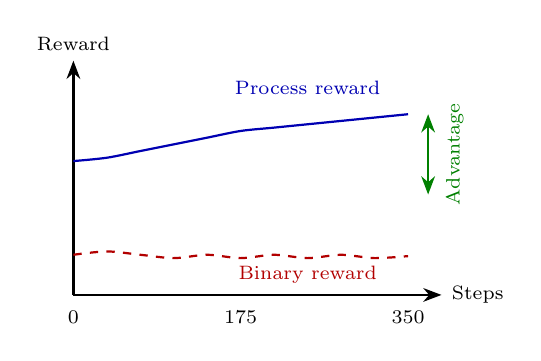
\begin{tikzpicture}[
    scale=0.85,
    every node/.style={font=\small},
  ]
  % Axes for reward curve
  \draw[-{Stealth}, thick] (0,0) -- (5.5,0) node[right] {\scriptsize Steps};
  \draw[-{Stealth}, thick] (0,0) -- (0,3.5) node[above] {\scriptsize Reward};

  % Process reward curve (increasing from ~1.01 to ~1.12)
  \draw[thick, blue!70!black] plot[smooth] coordinates {
    (0,2.0) (0.5,2.05) (1.0,2.15) (1.5,2.25) (2.0,2.35)
    (2.5,2.45) (3.0,2.5) (3.5,2.55) (4.0,2.6) (4.5,2.65) (5.0,2.7)
  };

  % Binary reward curve (flat/stagnant)
  \draw[thick, red!70!black, dashed] plot[smooth] coordinates {
    (0,0.6) (0.5,0.65) (1.0,0.6) (1.5,0.55) (2.0,0.6)
    (2.5,0.55) (3.0,0.6) (3.5,0.55) (4.0,0.6) (4.5,0.55) (5.0,0.58)
  };

  % Labels
  \node[blue!70!black, font=\scriptsize] at (3.5, 3.1) {Process reward};
  \node[red!70!black, font=\scriptsize] at (3.5, 0.3) {Binary reward};

  % Step markers
  \node[font=\scriptsize, below] at (0,-0.1) {0};
  \node[font=\scriptsize, below] at (2.5,-0.1) {175};
  \node[font=\scriptsize, below] at (5.0,-0.1) {350};

  % Advantage spread annotation
  \draw[{Stealth}-{Stealth}, thick, green!50!black] (5.3, 1.5) -- (5.3, 2.7);
  \node[green!50!black, font=\scriptsize, rotate=90] at (5.7, 2.1) {Advantage};
\end{tikzpicture}
\caption{GRPO training dynamics. Process reward enables steady improvement (reward mean: 1.01 $\to$ 1.12) with meaningful advantage spread ($-2.47$ to $+2.47$). Binary reward stagnates with near-zero spread.}
\label{fig:training}
\end{figure}

The process reward is \emph{necessary} for GRPO training on structured verification (Figure~\ref{fig:training}).
With binary reward, the reward distribution is bimodal ($\sim$1.38 vs.\ $\sim$0.02) with near-zero advantage spread, causing training to stagnate.

With process reward, training exhibits healthy dynamics:
\begin{itemize}[nosep,leftmargin=*]
  \item \textbf{Reward mean}: 1.01 $\to$ 1.12 over 350 steps
  \item \textbf{Entropy}: maintained at 0.06--0.21 (continued exploration)
  \item \textbf{Advantage spread}: $-2.47$ to $+2.47$ (effective gradient signal)
\end{itemize}

This demonstrates that process reward decomposition is essential for applying RL to structured output generation beyond mathematical reasoning.


\subsection{Ablation Study}

\begin{table}[t]
\centering
\small
\caption{Ablation on ClearFacts. SFT $\to$ GRPO with process reward accounts for the largest gain.}
\label{tab:ablation}
\begin{tabular}{lccc}
\toprule
\textbf{Configuration} & \textbf{F1} & \textbf{Align} & \textbf{Chain} \\
\midrule
\seva-GRPO (full) & \realnumber{69.0} & 0.997 & 0.995 \\
\midrule
$-$ GRPO (SFT only) & 64.9 & 0.917 & 0.917 \\
$-$ Process $\to$ binary reward & $<$65 & $<$0.92 & $<$0.92 \\
\bottomrule
\end{tabular}
\end{table}

Table~\ref{tab:ablation} shows the contribution of each component.
The largest gap is between SFT only and full GRPO (+4.1 F1), confirming that RL training provides substantial improvement for structured verification.
Replacing process reward with binary reward causes training to stagnate at SFT-level performance, validating that the reward decomposition is the key enabler.


\subsection{Qualitative Analysis}

\begin{figure}[t]
\centering
\small
\fbox{\parbox{0.95\columnwidth}{
\textbf{Claim:} ``60\% of participants significantly improved'' \\
\textbf{Source:} ``60\% of subjects showed improvement'' \\[4pt]
\textbf{\seva output:} \\
\texttt{evidence\_alignment:} \\
\quad ``60\% of participants'' $\to$ ``60\% of subjects'' [match] \\
\quad ``significantly improved'' $\to$ NOT\_FOUND [not\_found] \\[2pt]
\texttt{reasoning\_chain:} \\
\quad Step 1: ``60\% of participants'' --- supported (percentage matches) \\
\quad Step 2: ``significantly improved'' --- not\_supported (source says ``improvement'' without ``significantly'') \\[2pt]
\texttt{label:} Not Attributable \quad \texttt{confidence:} 0.85 \\
\texttt{error\_type:} scope\_inflation \\
\texttt{fix:} Change ``significantly improved'' to ``improved''
}}
\caption{\seva structured output example. The model identifies the specific mismatch, diagnoses \texttt{scope\_inflation}, and suggests a fix --- interpretability absent from binary verifiers.}
\label{fig:example}
\end{figure}

Figure~\ref{fig:example} illustrates \seva's interpretability advantage.
The model identifies the exact mismatch (``significantly improved'' vs.\ ``improved''), traces its reasoning step-by-step, and produces an actionable fix suggestion.
Binary verifiers provide none of this --- only a label.


\subsection{Error Analysis}

\begin{figure}[t]
\centering
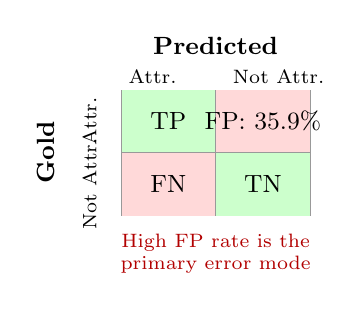
\begin{tikzpicture}[scale=0.8]
  % Confusion matrix
  \node[font=\small\bfseries] at (1.5, 3.2) {Predicted};
  \node[font=\small\bfseries, rotate=90] at (-1.2, 1.5) {Gold};

  \node[font=\scriptsize] at (0.5, 2.7) {Attr.};
  \node[font=\scriptsize] at (2.5, 2.7) {Not Attr.};
  \node[font=\scriptsize, rotate=90] at (-0.5, 2.0) {Attr.};
  \node[font=\scriptsize, rotate=90] at (-0.5, 1.0) {Not Attr.};

  % Cells
  \fill[green!20] (0,1.5) rectangle (1.5,2.5);
  \fill[red!15] (1.5,1.5) rectangle (3.0,2.5);
  \fill[red!15] (0,0.5) rectangle (1.5,1.5);
  \fill[green!20] (1.5,0.5) rectangle (3.0,1.5);

  \draw[black!40] (0,0.5) grid[step=1.5] (3.0,2.5);

  \node[font=\small] at (0.75, 2.0) {TP};
  \node[font=\small] at (2.25, 2.0) {FP: 35.9\%};
  \node[font=\small] at (0.75, 1.0) {FN};
  \node[font=\small] at (2.25, 1.0) {TN};

  % Annotation
  \node[font=\scriptsize, text=red!70!black, align=center] at (1.5, -0.1) {High FP rate is the\\primary error mode};
\end{tikzpicture}
\caption{Confusion pattern of \seva-GRPO on ClearFacts. The 35.9\% false positive rate (predicting ``Not Attributable'' for attributable claims) is the primary bottleneck.}
\label{fig:confusion}
\end{figure}

Detailed failure analysis (Figure~\ref{fig:confusion}) reveals that the dominant error mode is \emph{false positives}: \seva-GRPO incorrectly classifies 35.9\% of attributable claims as ``Not Attributable.''
This bias emerges because the model's error diagnosis component (which only activates for ``Not Attributable'' predictions) provides additional reward signal for negative predictions, creating an asymmetric incentive.
The format error rate also improved substantially: from 28\% (SFT) to near-zero (GRPO), demonstrating that the format reward component is effective.


% ==============================================================
\section{Discussion}
\label{sec:discussion}
% ==============================================================

\paragraph{Why process reward works.}
Process reward decomposes ``what makes a good verification'' into learnable sub-skills.
A model that learns to align evidence well receives reward even before learning correct label prediction.
This \emph{curriculum-like} effect allows GRPO to first master structural components, then improve label accuracy --- similar to how PRMs in math first reward correct intermediate steps.

\paragraph{Accuracy gap with larger verifiers.}
\seva-3B (69.0 F1) underperforms MiniCheck-7B (81.2 F1).
Three factors contribute: (1)~model capacity (3B vs.\ 7B); (2)~training data (5K structured vs.\ 57K binary annotations); (3)~output complexity (structured JSON vs.\ single token).
Scaling model size and training data are natural next steps; our framework is agnostic to both.

\paragraph{Interpretability--accuracy tradeoff.}
Requiring structured output imposes an overhead: the model must allocate capacity to producing well-formed spans and reasoning chains, potentially at the cost of classification accuracy.
However, this tradeoff is worthwhile in applications where \emph{why} matters as much as \emph{what} --- e.g., content moderation, medical claim verification, and legal document analysis.

\paragraph{Limitations.}
Our evaluation covers ClearFacts plus five auxiliary benchmarks; broader evaluation on LLM-AggreFact is needed.
The 5K training set is small; scaling annotation would improve results.
We evaluate only 3B models; scaling to 7--8B would enable fairer comparison with MiniCheck and ClearCheck.
The false-positive bias identified in our error analysis suggests that balanced reward calibration across label classes is an important direction.


% ==============================================================
\section{Conclusion}
\label{sec:conclusion}
% ==============================================================

We introduced \seva, a structured evidence verification framework with a process reward function that decomposes verification quality into five independently scored components.
On ClearFacts, \seva-3B improves +4.1 F1 from SFT to GRPO, with near-perfect structural quality (alignment: 0.997, chain: 0.995).
The process reward is essential: it creates a smooth optimization landscape that enables GRPO training for structured output, where binary reward fails entirely.
Across six benchmarks, \seva-GRPO shows strong gains on balanced verification tasks (FEVER, TruthfulQA) while revealing label bias as a key challenge for future work.
We release our code, reward function, and structured verification dataset.


% ==============================================================
% Ethics Statement
% ==============================================================
\section*{Ethics Statement}
\seva is designed to improve the reliability of AI systems by detecting unsupported claims.
We do not foresee significant negative societal impacts.
Our error taxonomy and fix suggestions are intended to help users correct --- not suppress --- information.
All training data is derived from publicly available benchmarks.

% ==============================================================
% Limitations
% ==============================================================
\section*{Limitations}
Our evaluation covers ClearFacts and five auxiliary benchmarks (200 samples each).
The model is trained on only 5K structured annotations.
We evaluate a single model size (3B) and do not yet compare at equal scale with 7--8B baselines.
The structured output format increases inference cost compared to binary-label verifiers.
The false-positive bias (35.9\%) identified in error analysis indicates that label-balanced reward calibration is needed.

% ==============================================================
% References
% ==============================================================
\bibliographystyle{acl_natbib}
\bibliography{references}

\end{document}
